\documentclass{article}
\usepackage[utf8]{vietnam}
\usepackage[12pt]{extsizes}
\usepackage{amsmath,amsfonts,amsthm}
\usepackage{mathrsfs}
\usepackage{enumitem}
\usepackage{geometry}
\usepackage{mathtools}
\usepackage{booktabs}
\usepackage{pgfplots}
\usepackage{amssymb}
\usepackage{array}
\usepackage{multirow}
\usepackage{tabularx}
\usepackage{hyperref}
\usepackage{mathrsfs}
\usepackage{float}
\pgfplotsset{compat=1.18}
 \geometry{
 a4paper,
 total={170mm,257mm},
 left=20mm,
 top=20mm,
 }
 \usepackage{graphicx}
 \usepackage{titling}
 \usepackage{listings}
 \title{Thiết kế bộ lọc IIR
}
\author{}
\date{Ngày 12/6/2025}
 \usepackage{fancyhdr}
\fancypagestyle{plain}{%  the preset of fancyhdr 
    \fancyhf{} % clear all header and footer fields
    \fancyfoot[L]{\thedate}
    \fancyhead[L]{}
    \fancyhead[R]{\theauthor}
}
\makeatletter\def\@maketitle{%
\newpage
\null
\vskip 1em%
\begin{center}%
\let \footnote \thanks
  {\LARGE \@title \par}%
  \vskip 1em%
  %{\large \@date}%
\end{center}%
\par
\vskip 1em}
\makeatother
\begin{document}
\maketitle
\section{Thiết kế bộ lọc tương tự}
\subsection{Thiết kế bộ lọc LP}
\subsubsection{Thiết kế bộ lọc Butterworth}
Bộ lọc Butterworth là bộ lọc "phẳng" nhất trong tất cả các họ bộ lọc, thế nhưng đổi lại là độ suy hao
(attenuation) của bộ lọc này thấp nhất (kéo theo transition band, band chuyển tiếp dài nhất). Ta quan sát đáp ứng biên độ của họ bộ lọc này và định nghĩa các tham số quan trọng sau:
\begin{figure}[H]
  \begin{center}
  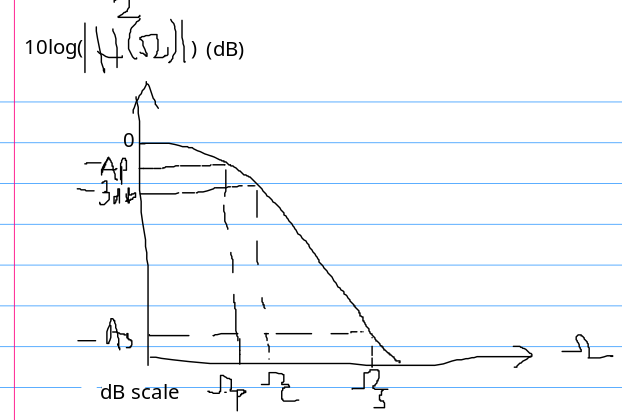
\includegraphics[width=10cm]{butter.png}
  \end{center}
  \end{figure}
  $$H(\Omega)^{2}=\frac{1}{1+(\frac{\Omega}{\Omega_{C}})^{2}}$$
$A_{P}$ là độ suy hao tại dải thông, $A_{s}$ là độ suy hao tại dải triệt (tính theo thang dB). $\Omega_{P}$ và
$\Omega_{S}$ lần lượt là tần số cắt tại dải thông và dải triệt. Lưu ý đặc biệt \textbf{đối với bộ lọc Butterworth thì $\Omega_{C}$ là
tần số góc tại điểm $A_{P}=3dB$} và chỉ duy nhất bộ lọc Butterworth có tính chất này. Tại $\Omega_{C}$ đó thì
độ suy hao của tín hiệu bắt đầu giảm nhanh. Nếu giả sử đề bài cho $0<f<10kHz \quad Ap<2.5dB$ thì tuyệt đối \textbf{không} được
kết luận ngay $f=10kHz$ là tần số cắt của bộ lọc, làm như vậy là sai.
\\ Giải pháp để xử lý các bài tập này anh đã gửi video lên rất nhiều lần và trong video có giải thích rất chi tiết
cách tính tần số cắt trong tình huống này. Không xem rồi nhỡ mà thi vào thì anh cũng chịu thua.
\subsubsection{Thiết kế bộ lọc Chebyshev}
Do yêu cầu của kì thi tương đối đơn giản nên ta chỉ xem xét bộ lọc Chebyshev loại I, tức là có gợn sóng ở dải thông. So với 
bộ lọc Butterworth thì bộ lọc Chebyshev tốt hơn nhiều do dải chuyển tiếp rất hẹp, nhưng bù lại là có gợn sóng.
\begin{figure}[H]
  \begin{center}
  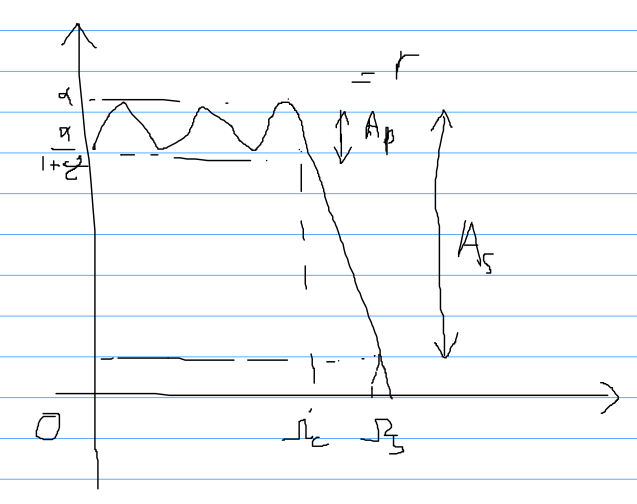
\includegraphics[width=10cm]{che.png}
  \end{center}
  \end{figure}
$$H(\Omega)^2=\frac{\alpha}{1+\varepsilon^2T_{N}^2(\frac{\Omega}{\Omega_{C}})}$$
Điểm khác biệt quan trọng nhất giữa bộ lọc Butterworth và Chebyshev đó là tần số cắt của bộ lọc Chebyshev không phải lúc nào cũng bằng $-3dB$ 
mà nó được định nghĩa là tần số mà ở đó bộ lọc kết thúc quá trình ripples. Phần còn lại rất dễ và tự ôn nốt.
\subsection{Thiết kế bộ lọc BP}
Đối với bộ lọc Analog, chúng ta đều thiết kế tất cả các bộ lọc khác dựa trên bộ lọc LP bằng phương pháp
mapping (ánh xạ) như sau:
\\ Ta định nghĩa các biến mới như sau:
\begin{figure}[H]
  \begin{center}
  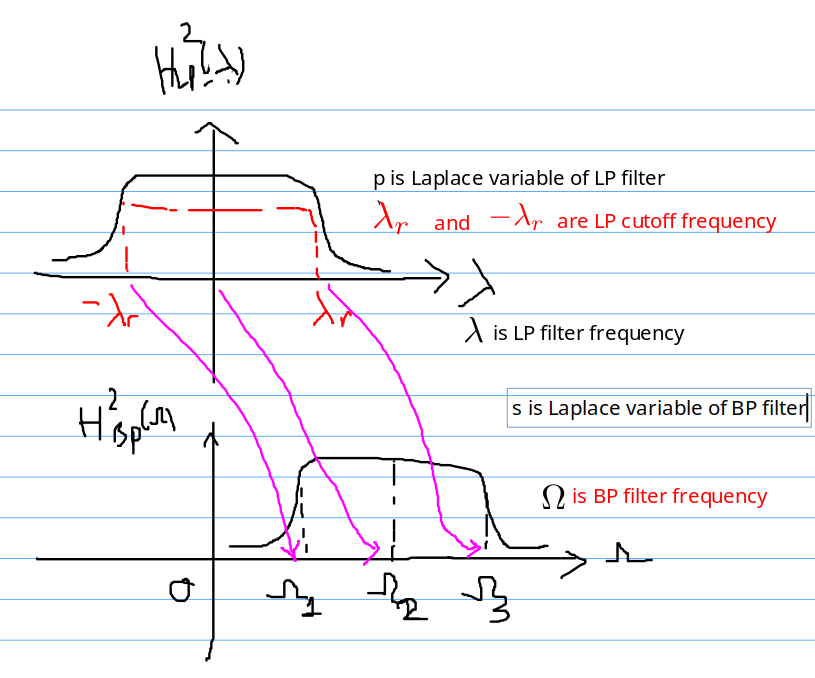
\includegraphics[width=16cm]{10.png}
  \end{center}
  \end{figure}
Đối với chuyển đổi từ bộ lọc LP sang BP, ta có công thức sau (đã được anh giải thích từ hồi ôn IIR thi giữa kì):
\begin{equation*}
    \begin{split}
        p=\frac{s^2+\Omega_{2}^2}{s}\rightarrow \lambda=\frac{\Omega^2-\Omega_{2}^2}{\Omega}
    \end{split}
\end{equation*}
Đây là công thức liên hệ giữa tần số của cả $2$ bộ lọc LP và BP. Tiếp theo, ta sẽ tiến hành mapping $-\lambda_{r}$ với $\Omega_{1}$ và $\lambda_{r}$ với $\Omega_{3}$.
\begin{equation*}
    \begin{split}
        -\lambda_{r}&=\frac{\Omega_{1}^2-\Omega_{2}^2}{\Omega_{1}}\rightarrow -F_{r}=\frac{F_{1}^2-F_{2}^2}{F_{1}}\\
        \lambda_{r}&=\frac{\Omega_{3}^2-\Omega_{2}^2}{\Omega_{3}}\rightarrow F_{r}=\frac{F_{3}^2-F_{2}^2}{F_{3}}\\
    \end{split}
\end{equation*}
Biến đổi tương đương, ta thu được $F_{r}=F_{3}-F_{1}$ và $F_{2}=\sqrt{F_{1}F_{3}}$. Vậy ta xây dựng thuật toán gồm 3 bước
sau để tạo ra bộ lọc BP tương ứng:
\begin{enumerate}
    \item Tính tần số cắt của bộ lọc LP và tần số trung tâm của bộ lọc BP bằng công thức:
    $$F_{r}=F_{3}-F_{1} \quad F_{2}=\sqrt{F_{1}F_{3}}$$
    \item Xây dựng bộ lọc LP tương ứng có tần số cắt $F_{r}$.
    \item Chuyển bộ lọc LP về BP bằng công thức:
    $$p=\frac{s^2+\Omega_{2}^2}{s}$$
\end{enumerate}
Tất nhiên là đi thi sẽ không bao giờ có chuyện dễ và ngon ăn như thế này (xem bài tập của Linh Trung là hiểu), vì ở đây anh chưa xét đến yếu tố $A_{stop}$ của
bộ lọc mà thôi. Cách xử lý với trường hợp có yếu tố $A_{stop}$ là dùng công thức chuyển tần số của BP về LP để tiếp tục xử lý trong các bài 
yêu cầu thiết kế bộ lọc bằng phương pháp đáp ứng xung hay đáp ứng nhảy bậc. Bài của Lưu Mạnh Hà thì đã có đầy đủ ví dụ trong slide, anh chỉ
viết lại lý thuyết sao cho trông nó "humanable" nhất có thể thôi.
\subsection{Thiết kế bộ lọc BS}
Tương tự như bộ lọc BP, chỉ khác một chút ở cách mapping
\begin{figure}[H]
  \begin{center}
  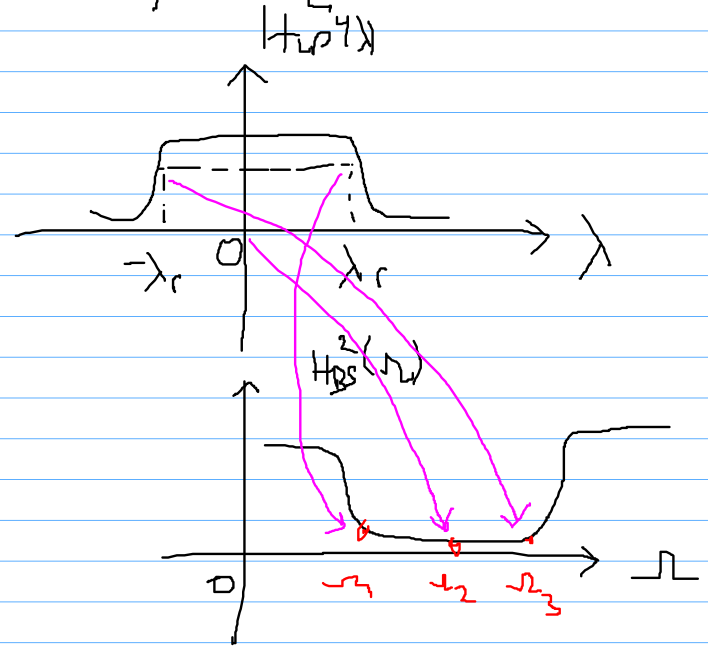
\includegraphics[width=16cm]{12.png}
  \end{center}
  \end{figure}
Kí hiệu và đơn vị quy ước giống hệt ở trên, anh không nhắc lại nữa. Công thức chuyển đổi từ bộ lọc LP sang BS như sau:
$$p=\frac{\Omega_{2}^2s}{s^2+\Omega^2}\rightarrow \lambda=\frac{\Omega_{2}^2\Omega}{\Omega_{2}^2-\Omega^2}$$
Mapping theo như hình vẽ, ta có: $$\frac{\lambda_{r}}{2\pi}=\frac{F_{2}^2F_{1}}{F_{2}^2-F_{1}^2}$$
$$\frac{-\lambda_{r}}{2\pi}=\frac{F_{2}^2F_{3}}{F_{2}^2-F_{3}^2}$$
Biến đổi tương đương một chút (tự làm), thu được $F_{2}=\sqrt{F_{1}F_{3}}$ và $$B=F_{3}-F_{1}=\frac{F_{1}F_{3}}{F_{r}}\rightarrow F_{r}=\frac{F_{3}F_{1}}{F_{3}-F_{1}}$$
Vậy ta cũng phát triển được thuật toán để chuyển bộ lọc LP về BS như sau:
\begin{enumerate}
    \item Tính tần số cắt của bộ lọc LP và tần số trung tâm của bộ lọc BS theo công thức ở trên.
    \item Xây dựng bộ lọc LP tương ứng có tần số cắt $F_{r}$
    \item Chuyển bộ lọc LP về BS bằng công thức:
    $$p=\frac{\Omega_{2}^2s}{s^2+\Omega^2}$$
\end{enumerate}
\subsection{Thiết kế bộ lọc HP}
Bộ lọc HP có cách mapping khá đặc biệt như sau:
\begin{figure}[H]
  \begin{center}
  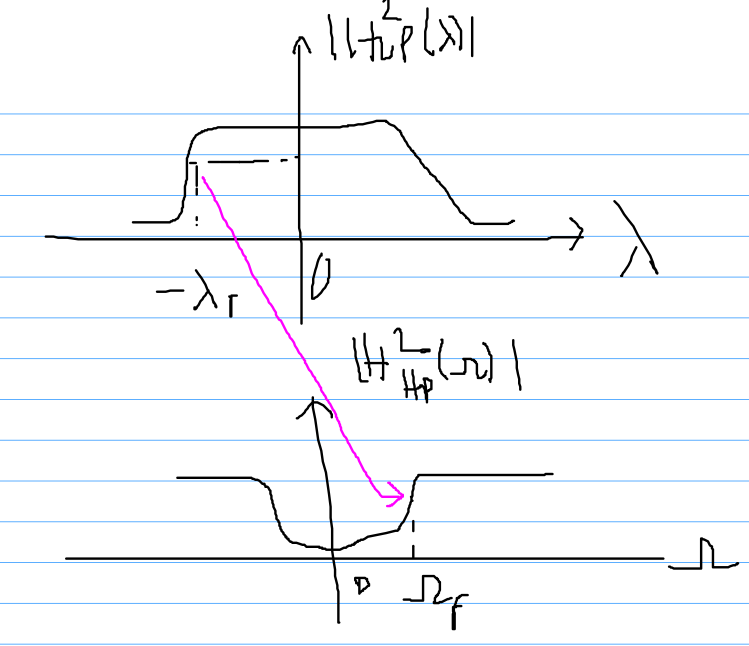
\includegraphics[width=14cm]{13.png}
  \end{center}
  \end{figure}
Công thức mapping là:
$$p=\frac{\lambda_{r}\Omega_{r}}{s}\rightarrow \lambda=\frac{-\lambda_{r}\Omega_{r}}{\Omega}$$
Ta cũng có thuật toán gồm 2 bước để xây dựng họ bộ lọc HP như sau:
\begin{enumerate}
    \item Thu được tần số cắt $\lambda_{r}=\Omega_{r}$ của bộ lọc LP tương tự (tương đương với bước mapping).
    \item Chuyển bộ lọc LP thu được về HP qua công thức $$p=\frac{\lambda_{r}\Omega_{r}}{s}$$
\end{enumerate}
\textbf{Nếu thi gặp phải các yếu tố như $A_{stop}$ hay tần tại dải triệt thì xử lý bằng công thức đổi dải tần, rồi làm LP Butter hoặc Cheb như bình thường rồi đổi lại về bộ lọc mong muốn.}
\section{Thiết kế bộ lọc số}
\subsection{Thiết kế bằng phương pháp đáp ứng xung bất biến hoặc đáp ứng bậc thang}
Công thức đáp ứng xung bất biến:
$$H(s)=\sum\frac{c_{i}}{s-\lambda_{i}} \rightarrow H(z)=\sum T_{s}\frac{c_{i}z}{z-e^{\lambda_{i}T_{s}}}$$
Công thức đáp ứng bậc thang:
$$H(s)=\sum\frac{c_{i}}{s-\lambda_{i}} \rightarrow H(z)=\sum \frac{1}{\lambda_{i}}\frac{c_{i}(e^{\lambda_{i}T_{s}}-1)}{z-e^{\lambda_{i}T_{s}}}$$
Công thức liên hệ tần số số (digital) và tần số tương tự (analog) đã được thảo luận kĩ ở lần ôn thi IIR giữa kì trước và đã học hết lại toàn bộ từ
đầu cách thiết kế các bộ lọc Analog ở trên. Lưu ý là \textbf{cách của cô Thịnh khá là không chặt chẽ và không thể dùng cho rất nhiều trường hợp nên phải học lại cách/ý tưởng thiết kế của ông Linh Trung từ đầu.}
\subsection{Thiết kế bằng phương pháp song tuyến tính}
\subsubsection{Ý tưởng của phương pháp song tuyến tính}
Hoàn toàn giống hệt với phép mapping bộ lọc Analog đã thảo luận ở trên, phương pháp song tuyến tính sử dụng để map giữa tần số trong miền tương tự và tần số
trong miền số với nhau.
Phép mapping này có công thức như sau:
$$p=C\frac{1-z^{-1}}{1+z^{-1}}$$ $$\Omega=C\tan{\frac{\omega}{2}}$$
Lưu ý rằng quy ước biến Laplace $p$ hoàn toàn giống với quy ước biến của phép mapping bộ lọc Analog đã được thảo luận ở trên. Vậy nên
\textbf{khác hoàn toàn với cách của cô Thịnh khi phải map của bộ lọc trung gian, phép mapping này tối ưu hơn rất nhiều khi tiết kiệm được một bước thừa thãi, cho ra kết quả rất chính xác vì mình muốn map ở đâu thì map và đây cũng chính
là cách MatLab được lập trình để thiết kế các bộ lọc số. Nếu có thời gian và có hứng thú, em nên thử tự thiết kế lại bộ lọc trong MatLab và so sánh hệ số [b a] với kết quả tính tay.}
\\ Ở đây ta sẽ quy ước một khái niệm mới, đó là tần số số như sau:
$$v=\frac{F}{F_{N}}$$
nhưng như anh đã giải thích tối hôm qua \textit{đây chỉ là cách quy ước theo MatLab được lập trình để thiết kế bộ lọc số, chứ không phải là định nghĩa chính xác của tần số số}
\subsubsection{Thiết kế bộ lọc LP}
\begin{figure}[H]
  \begin{center}
  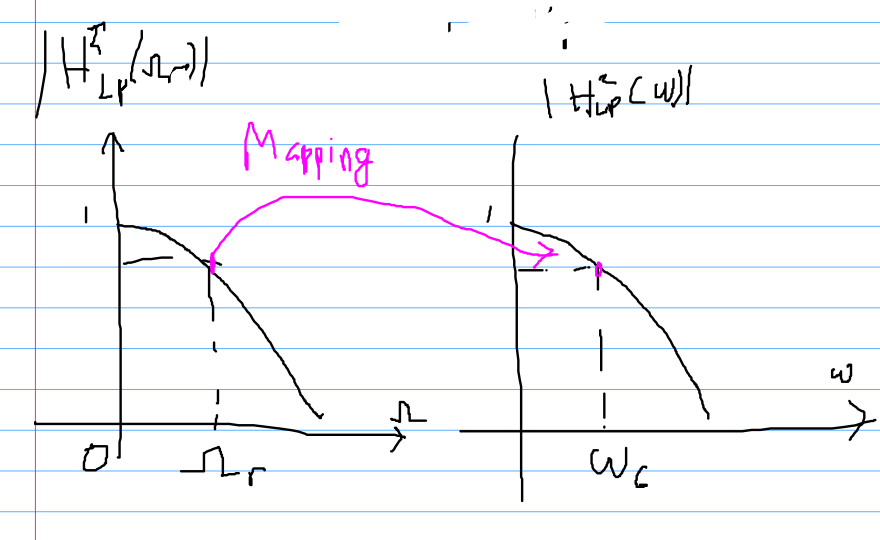
\includegraphics[width=13cm]{15.png}
  \end{center}
  \end{figure}
Theo như định nghĩa ở trên, ta có công thức sau:
$$\Omega=C\tan\left(\frac{\omega}{2}\right)=C\tan\left(\frac{\pi F}{F_{sam}}\right)=C\tan{\left(\frac{\pi F}{2F_{N}}\right)}=C\tan{\left(\frac{\pi}{2}v\right)}$$
Đối với bộ lọc LP, chúng ta sẽ map giữa $\Omega_{r}\rightarrow v_{r}$ như sau:
$$C=\Omega_{r}\cot{\left(\frac{\pi}{2}v_{r}\right)}$$
Một lựa chọn rất thông minh ở đây đó là thay vì map giữa các dải tần ngẫu nhiên ta sẽ map ngay tại tần số chuẩn hóa của bộ lọc LP analog là $\Omega_{r}=1\; (rad/s)$, vậy ta
đã chọn được hằng số $C$ sao cho $\Omega_{r}=1\; (rad/s)\rightarrow v_{r}$. Ta đã thành công tính được hằng số $C$, việc còn lại chỉ là map lần lượt từng tần số $v$ qua $\Omega$ để giải quyết bài toán
và cuối cùng dùng phép biến đổi:
$$p=C\frac{1-z^{-1}}{1+z^{-1}}$$ 
để chuyển lại bộ lọc analog về bộ lọc digital.
\subsubsection{Thiết kế bộ lọc BP}
Quy trình thiết kế bộ lọc bandpass tương đối phức tạp khi phải đi qua một bộ lọc trung gian ở giữa, nhưng các công thức đã được cho (và không chứng minh) trong slide gốc
có thể được áp dụng và hiểu về nguyên lý hoạt động như sau:
\begin{figure}[H]
  \begin{center}
  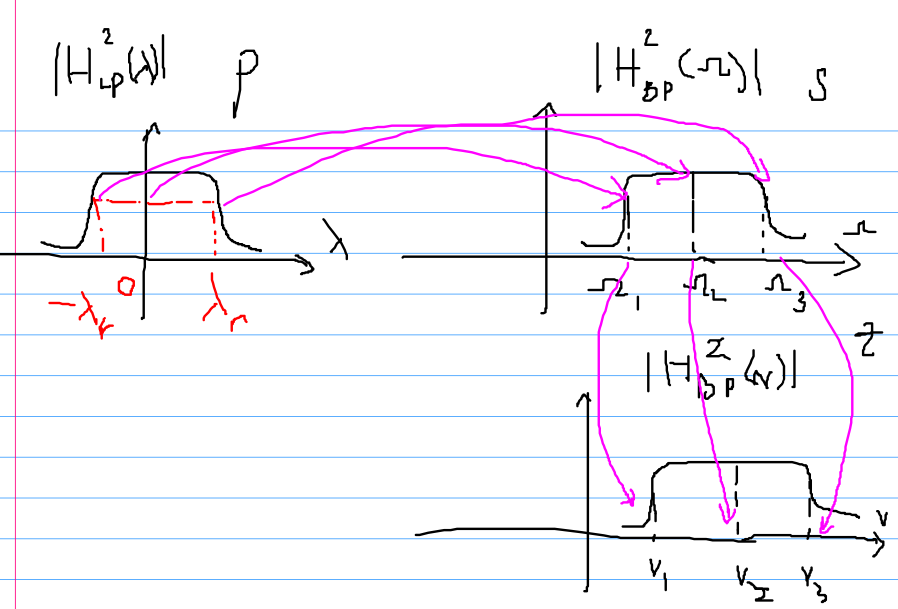
\includegraphics[width=13cm]{16.png}
  \end{center}
  \end{figure}
Quan sát quy trình trên ta có thể thấy phải mapping qua một bộ lọc $H_{BP}(\Omega)$ trung gian chứ không map trực tiếp từ $p\to z$ được. Ta đã có các kết quả sau (công nhận):
\begin{equation*}
  \begin{split}
  p&=D\frac{1-Ez^{-1}+z^{-2}}{1+z^{-2}}\\
  D&=\lambda_{r}\cot{\left(\frac{\pi}{2}(v_{3}-v_{1})\right)}\\
  E&=\frac{2\cos{\left(\frac{\pi}{2}(v_{3}-v_{1})\right)}}{\cos{\left(\frac{\pi}{2}(v_{3}+v_{1})\right)}}\\
  \lambda&=D\frac{\cos{(\pi v_{2})}-\cos{(\pi v)}}{\sin{(\pi v)}}
  \end{split}
\end{equation*}
Và kết quả đã được chứng minh từ phần bộ lọc BP Analog, ta cũng có:
$$\Omega_{2}^2=\Omega_{1}\Omega_{3}\to \tan^2{\left(\frac{\pi v_{2}}{2}\right)}=\tan{\left(\frac{\pi v_{1}}{2}\right)}\tan{\left(\frac{\pi v_{3}}{2}\right)}$$
Ý tưởng giống như thiết kế bộ lọc LP, đầu tiên ta sẽ khống chế $\lambda_{r}=1 \; (rad/s)$ để đưa bộ lọc LP về bộ lọc có tần cắt chuẩn hóa. Từ các thông số $v_{1}, v_{3}$
đã cho ở đầu bài ta sẽ tính được ngay $v_{2}$ và $D, E$. Công thức $\lambda$ cuối cùng sử dụng để chuyển các tần số từ thang $v$ (thang tần số số) về thang $\lambda$ (thang tần số tương tự của bộ lọc LP chuẩn hóa). Nếu em thử thay $v_{1}$ và $v_{3}$ vào công thức
này chắc chắn kết quả sẽ ra tương ứng là $1$ và $-1$. Cuối cùng, thay ngược $D, E$ vào $p$, ta thu được bộ lọc thông dải cần tìm.
\subsubsection{Thiết kế bộ lọc BS}
Hiện tại, trong sách/slide gốc thì phần BS này đang bị thiếu công thức để chuyển từ dải tần tần số số về tần số tương tự chuẩn hóa nên hy vọng hôm thi sẽ không
hỏi cái này.
\begin{equation*}
  \begin{split}
  p&=D\frac{1+z^{-2}}{1-Ez^{-1}+z^{-2}}\\
  D&=\lambda_{r}\tan{\left(\frac{\pi}{2}(v_{3}-v_{1})\right)}\\
  E&=\frac{2\cos{\left(\frac{\pi}{2}(v_{3}+v_{1})\right)}}{\cos{\left(\frac{\pi}{2}(v_{3}-v_{1})\right)}}\\
    \end{split}
\end{equation*}
\subsubsection{Thiết kế bộ lọc HP}
Lưu ý, thiết kế bộ lọc HP rất giống với LP, nhưng chỉ khác là các công thức bị \textbf{"lộn" ngược lại.}
\begin{figure}[H]
  \begin{center}
  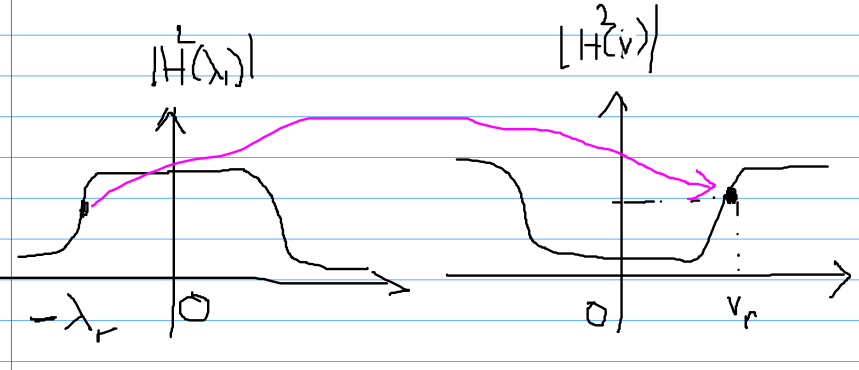
\includegraphics[width=13cm]{30.png}
  \end{center}
  \end{figure}
  $$\lambda=C\cot{\left(\frac{\omega}{2}\right)} \to C=\lambda \tan{\left(\frac{\pi v}{2}\right)}$$
  $$p=C\frac{1+z^{-1}}{1-z^{-1}}$$
Đặt $\lambda_{r}=1$, tìm C rồi làm tương tự như LP.
\section{Bài tập áp dụng (thiết kế bộ lọc LP như giới hạn thi)}
\begin{enumerate}
  \item Đổi tất cả tần số ở miền digital sang tần số số $v$. Xác định $v_{r}$ (tần cắt số ở miền số).
  \item Xác định hằng số $C$ để map giữa tần cắt miền số $v_{r}$ với tần cắt chuẩn hóa ở miền tương tự $\Omega_{r}=1\; (rad/s)$.
  \item Dùng hằng số $C$ đã tìm được ở trên để tiếp tục map $v_{s}$ với tần số dừng ở miền tương tự $\Omega_{s}$.
  \item Thiết kế bộ lọc tương tự theo các đặc tả (characteristics) đã xác định ở bước $3$ và đề bài.
  \item Chuyển bộ lọc tương tự về bộ lọc số thông qua phép đổi biến $p\to z$.
\end{enumerate}
\subsection{Thiết kế bộ lọc LP Butterworth bằng phương pháp song tuyến tính với $A_{p}<3\; dB$ với $0<F<25\; Hz$ và 
$A_{p}>38dB$ với $F>50Hz$; $Fsam=200\; Hz.$}
$$v_{r}=\frac{F_{r}}{F_{N}}=0.25\quad v_{s}=\frac{F_{s}}{F_{N}}=0.5$$
Sử dụng phương pháp song tuyến tính, ta chọn hằng số $C$ để map giữa tần số cắt chuẩn hóa của bộ lọc tương tự đến tần số số $v_{r}$
$$C=\Omega_{r}\cot{\left(\frac{\pi}{2}v_{r}\right)}=\cot{\left(\frac{\pi}{2}v_{r}\right)}=2.4142$$
Vậy ta sẽ map tần số $v_{s}$ sang miền tần số tương tự như sau:
$$\Omega_{s}=C\tan{\left(\frac{\pi}{2}v_{s}\right)}=2.4142 \quad (rad/s)$$
Ý nghĩa của phép biến đổi song tuyến tính này là chúng ta chọn hằng số $C$ để map các đại lượng như sau:
$$v_{r}=0.25\to \Omega_{c}=1$$ $$v_{s}=0.5\to \Omega_{s}=2.4142$$
Vậy bài toán được đưa về thiết kế bộ lọc tương tự Butterworth thỏa mãn các đặc tả trên. Ta tính được chỉ số tần số chuẩn hóa (Normalized Frequency):
$$NF=\frac{\Omega_{s}}{\Omega_{c}}=2.4142$$
Nhìn đồ thị, ta chọn được bộ lọc Butterworth có bậc: $N=5$.
Ta sẽ thiết kế được bộ lọc LP chuẩn hóa bậc $5$ như sau:
$$H(p)=\frac{1}{B_{5}(p)}=\frac{1}{\dots}$$
Bước cuối cùng, thay biến $p\to z$ theo công thức là xong:
$$p=C\frac{1-z^-1}{1+z^-1}$$
\subsection{Thiết kế bộ lọc Butterworth số bậc 3 với tần số cắt $\omega_{c}=0.15\pi$ và tần số lấy mẫu là $6kHz$}
\subsubsection{Tính $H(s)$ của bộ lọc tương tự}
$$H(s)=\frac{1}{B_{3}(s)}=\frac{1}{(s+1)(s^2+s+1)}$$
\subsubsection{Thiết kế bằng phương pháp bất biến xung}
Đổi tần cắt số sang tần cắt tương tự: $\Omega_{c}=\omega_{c}F_{sam}=900\pi$, từ đây ta có phương trình của bộ lọc $H_{LP}(s)$ với tần cắt trên:
$$H_{LP}(s)=\frac{1}{\left(\frac{s}{\Omega_{c}}+1\right)\left(\frac{s^2}{\Omega_{c}^2}+\frac{s}{\Omega_{c}}+1\right)}=\frac{\Omega_{c}^3}{(s+\Omega_{c})(s^2+s \Omega_{c}+\Omega_{c}^2)}$$
\subsubsection{Thiết kế bằng phương pháp song tuyến tính}
Đổi tần số $\omega_{c}$ sang miền tần số số:
$$\omega=\frac{2\pi F}{F_{s}}=\frac{\pi F}{F_{N}}=\pi v \Rightarrow v=0.15 $$
Chọn C để map giữa tần số cắt $v_{c}$ sang tần số cắt của bộ lọc LP tương tự đã chuẩn hóa:
$$C=\Omega \cot{\left(\frac{\pi v}{2}\right)}=4.1653$$
Do bậc bộ lọc số là bậc 3 nên ta suy ra bậc của bộ lọc tương tự cũng là bậc 3, vậy ta có hàm truyền của bộ lọc LP tương tự đã chuẩn hóa:
$$H(s)=\frac{1}{(s+1)(s^2+s+1)}$$
Bước cuối cùng là thay 
$$s=C\frac{1-z^-1}{1+z^-1}$$ vào $H(s)$ là xong.
\end{document}